% ConfigStream checkpoint deck -- redesigned, source-evidence scoped
% Build: latexmk -pdf -interaction=nonstopmode ConfigStream_Checkpoint_Redesigned.tex
% 16:9, self-contained: diagrams and charts are generated in LaTeX / TikZ.
\documentclass[aspectratio=169,10pt]{beamer}
\usepackage[T1]{fontenc}
\usepackage[utf8]{inputenc}
\usepackage{lmodern}
\usepackage{microtype}
\usepackage{graphicx}
\usepackage{booktabs}
\usepackage{array}
\usepackage{tabularx}
\usepackage{amsmath,amssymb}
\usepackage{tikz}
\usetikzlibrary{arrows.meta,positioning,calc,fit,backgrounds,shapes.geometric}
\usepackage[most]{tcolorbox}
\usepackage{hyperref}
\usepackage{xcolor}
\usepackage{colortbl}

\definecolor{Navy}{HTML}{152940}
\definecolor{Navy2}{HTML}{203D59}
\definecolor{Teal}{HTML}{007F83}
\definecolor{Mint}{HTML}{D9F2ED}
\definecolor{Blue}{HTML}{2476A8}
\definecolor{Sky}{HTML}{EAF3F9}
\definecolor{Gold}{HTML}{B78023}
\definecolor{PaleGold}{HTML}{FCF3DF}
\definecolor{Red}{HTML}{B84C4C}
\definecolor{PaleRed}{HTML}{FBEBE9}
\definecolor{Dark}{HTML}{192C3B}
\definecolor{Muted}{HTML}{607284}
\definecolor{Line}{HTML}{D5DFE6}
\definecolor{Paper}{HTML}{F7FAFC}
\definecolor{White}{HTML}{FFFFFF}

\setbeamercolor{background canvas}{bg=Paper}
\setbeamercolor{normal text}{fg=Dark}
\setbeamercolor{frametitle}{fg=Navy}
\setbeamerfont{frametitle}{size=\fontsize{22}{25}\selectfont,series=\bfseries}
\setbeamersize{text margin left=0.56cm,text margin right=0.56cm}
\setbeamertemplate{navigation symbols}{}
\setbeamertemplate{headline}{}
\setbeamertemplate{frametitle}{%
  \vspace{0.19cm}\hspace{0.55cm}\insertframetitle\par
  \vspace{0.055cm}\hspace{0.56cm}{\color{Teal}\rule{1.0cm}{2.2pt}}\par\vspace{0.06cm}}
\setbeamertemplate{footline}{%
 \leavevmode\hbox{\begin{beamercolorbox}[wd=.68\paperwidth,ht=.29cm,dp=.13cm,leftskip=.58cm]{normal text}%
 {\fontsize{7}{8}\selectfont\color{Muted}CONFIGSTREAM  /  GROUP 4  /  CHECKPOINT 01}%
 \end{beamercolorbox}\begin{beamercolorbox}[wd=.32\paperwidth,ht=.29cm,dp=.13cm,rightskip=.52cm plus1fil]{normal text}%
 \hfill{\fontsize{7}{8}\selectfont\color{Muted}26 OCT 2026\quad \insertframenumber/\inserttotalframenumber}%
 \end{beamercolorbox}}}

\tcbset{enhanced,boxrule=.45pt,arc=2.7mm,left=3mm,right=3mm,top=1.15mm,bottom=1.15mm,
        colback=White,colframe=Line,boxsep=0mm}
\newcommand{\strong}[1]{{\color{Navy}\bfseries #1}}
\newcommand{\muted}[1]{{\color{Muted}#1}}
\newcommand{\kicker}[1]{{\fontsize{10}{12}\selectfont\color{Teal}\bfseries\MakeUppercase{#1}}}
\newcommand{\sourceline}[1]{%
\begin{tikzpicture}[remember picture,overlay]
\node[anchor=south west,text width=12.0cm,align=left,font=\fontsize{6.0}{7.1}\selectfont,text=Muted] at ([xshift=.56cm,yshift=.50cm]current page.south west) {SOURCE / SCOPE: #1};
\end{tikzpicture}}
\newcommand{\bottomline}[1]{\vspace{.12cm}\begin{tcolorbox}[colback=Sky,colframe=Sky,arc=1.4mm,top=1mm,bottom=1mm]\fontsize{9}{11}\selectfont\strong{#1}\end{tcolorbox}}
\newcommand{\bigstat}[3]{\begin{tcolorbox}[colback=#3,colframe=#3,arc=2mm,halign=center]
 {\fontsize{21}{24}\selectfont\bfseries\color{Navy}#1}\par\vspace{1mm}{\fontsize{8}{10}\selectfont\color{Muted}#2}\end{tcolorbox}}
\tikzset{flow/.style={draw=Line,rounded corners=3pt,fill=White,minimum height=.8cm,align=center,font=\fontsize{9}{11}\selectfont,text=Dark,inner sep=5pt},
  darkflow/.style={flow,fill=Navy,text=White,draw=Navy},
  tealflow/.style={flow,fill=Mint,draw=Teal},
  flowarrow/.style={-Latex,thick,draw=Teal}}
\hypersetup{colorlinks=true,urlcolor=Blue,pdfauthor={ConfigStream Group 4},
 pdftitle={ConfigStream - Architecture-First Milestone Checkpoint}}

\begin{document}

\begin{frame}[plain]
\begin{tikzpicture}[remember picture,overlay]
  \fill[Navy] (current page.south west) rectangle (current page.north east);
  \fill[Navy2] ([xshift=8.3cm]current page.south west) -- (current page.south east)
      -- (current page.north east) -- ([xshift=10.5cm]current page.north west) -- cycle;
  \draw[Teal,line width=5pt] ([xshift=0.78cm,yshift=-0.83cm]current page.north west) -- ++(1.0,0);
  \node[anchor=west,text=White,font=\fontsize{36}{42}\selectfont\bfseries] at ([xshift=.78cm,yshift=-2.1cm]current page.north west) {ConfigStream};
  \node[anchor=west,text=White,font=\fontsize{17}{20}\selectfont] at ([xshift=.80cm,yshift=-3.02cm]current page.north west) {Architecture for trustworthy temporal history};
  \node[anchor=west,text=Mint,font=\fontsize{11}{14}\selectfont] at ([xshift=.80cm,yshift=-3.62cm]current page.north west) {Kafka, stateful Spark, committed Parquet and explainable queries};
  \node[anchor=west,text=White,font=\fontsize{10}{13}\selectfont] at ([xshift=.80cm,yshift=-5.35cm]current page.north west) {Group 4  |  Big Data Storage \& Processing};
  \node[anchor=west,text=White,font=\fontsize{9}{11}\selectfont] at ([xshift=.80cm,yshift=-5.75cm]current page.north west) {Ph\d am C\^ong Ho\`ang  \quad L\^e Ti\'en H\d op  \quad Mai V\~u Ho\`ang  \quad Nguy\~en \DJ\'uc D\~ung};
  \node[anchor=west,text=Mint,font=\fontsize{9}{12}\selectfont] at ([xshift=.80cm,yshift=-6.50cm]current page.north west) {FIRST MILESTONE  /  26 OCTOBER 2026};
  \foreach \x/\y/\r in {10.0/2.0/.10,10.8/2.8/.07,11.6/3.8/.13,9.2/4.7/.09,12.15/5.8/.07}{
    \fill[Teal!65] (\x,\y) circle (\r);
  }
  \draw[Mint!70,line width=1.3pt] (9.2,4.7)--(10.0,2.0)--(10.8,2.8)--(11.6,3.8)--(12.15,5.8);
\end{tikzpicture}
\end{frame}

\begin{frame}{Configuration change: before and after}
\vspace{.11cm}
\begin{columns}[T,onlytextwidth]
\begin{column}{.49\textwidth}
\begin{tcolorbox}[colback=White,title={\color{Navy}\bfseries Router R-001 / version 10},coltitle=Navy,colbacktitle=Sky]
{\ttfamily\fontsize{11}{14}\selectfont
hostname router-001\\
logging \textcolor{Teal}{enabled}\\
telnet \textcolor{Teal}{disabled}}
\par\medskip\muted{20 Oct 2026  /  08:00 UTC}
\end{tcolorbox}
\end{column}
\begin{column}{.49\textwidth}
\begin{tcolorbox}[colback=White,title={\color{Navy}\bfseries Router R-001 / version 11},coltitle=Navy,colbacktitle=PaleRed]
{\ttfamily\fontsize{11}{14}\selectfont
hostname router-001\\
logging \textcolor{Red}{disabled}\\
telnet \textcolor{Red}{enabled}}
\par\medskip\muted{20 Oct 2026  /  09:00 UTC}
\end{tcolorbox}
\end{column}
\end{columns}
\vspace{.18cm}
\begin{tcolorbox}[colback=Sky,colframe=Sky]
\centering \fontsize{17}{20}\selectfont\strong{What changed?} \quad \strong{When?} \quad \strong{On which asset?}
\end{tcolorbox}
\vspace{.13cm}
\fontsize{10}{13}\selectfont A latest-state file cannot answer these questions without versioned evidence and comparison logic.
\sourceline{Illustrative example adapted from processing/demo.py; timestamps are explanatory, not source measurements.}
\end{frame}

\begin{frame}{The product: three linked capabilities}
\vspace{.10cm}
\begin{columns}[T,onlytextwidth]
\begin{column}{.32\textwidth}\begin{tcolorbox}[height=3.2cm,colback=Sky,colframe=Sky]
\centering\vspace{.25cm}{\fontsize{30}{34}\selectfont\color{Blue}\bfseries 01}\\[3mm]
\strong{Preserve history}\\[2mm]
{\fontsize{9}{12}\selectfont Snapshots with identity, version, time and provenance}
\end{tcolorbox}\end{column}
\begin{column}{.32\textwidth}\begin{tcolorbox}[height=3.2cm,colback=Mint,colframe=Mint]
\centering\vspace{.25cm}{\fontsize{30}{34}\selectfont\color{Teal}\bfseries 02}\\[3mm]
\strong{Explain changes}\\[2mm]
{\fontsize{9}{12}\selectfont Compare adjacent versions and evaluate explicit rules}
\end{tcolorbox}\end{column}
\begin{column}{.32\textwidth}\begin{tcolorbox}[height=3.2cm,colback=PaleGold,colframe=PaleGold]
\centering\vspace{.25cm}{\fontsize{30}{34}\selectfont\color{Gold}\bfseries 03}\\[3mm]
\strong{Search \& analyze}\\[2mm]
{\fontsize{9}{12}\selectfont Query safe metadata and study temporal patterns}
\end{tcolorbox}\end{column}
\end{columns}
\vspace{.26cm}
\begin{tcolorbox}[colback=White]
\strong{Core design question}\quad How do we preserve correct temporal meaning under retries, late arrivals and failures?
\end{tcolorbox}
\sourceline{schemas/; processing/; spark/streaming/; api/routes/documents.py.}
\end{frame}

\begin{frame}{End-to-end architecture: configuration path}
\vspace{-.02cm}
\begin{center}
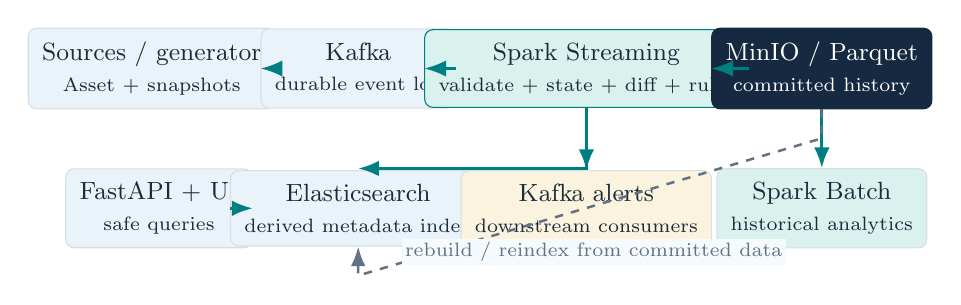
\begin{tikzpicture}[x=.92cm,y=.92cm,>=Latex,every node/.style={align=center}]
\node[flow,fill=Sky,minimum width=2.12cm,minimum height=.84cm] (producer) at (0.85,2.95) {Sources / generator\\\scriptsize Asset + snapshots};
\node[flow,fill=Sky,minimum width=1.92cm,minimum height=.84cm] (kafka) at (3.70,2.95) {Kafka\\\scriptsize durable event log};
\node[tealflow,minimum width=2.24cm,minimum height=.84cm] (spark) at (6.85,2.95) {Spark Streaming\\\scriptsize validate + state + diff + rules};
\node[darkflow,minimum width=2.26cm,minimum height=.84cm] (lake) at (10.10,2.95) {MinIO / Parquet\\\scriptsize committed history};

\node[flow,fill=Sky,minimum width=1.98cm,minimum height=.70cm] (api) at (0.95,1.02) {FastAPI + UI\\\scriptsize safe queries};
\node[flow,fill=Sky,minimum width=2.18cm,minimum height=.70cm] (es) at (3.70,1.02) {Elasticsearch\\\scriptsize derived metadata index};
\node[flow,fill=PaleGold,minimum width=2.12cm,minimum height=.70cm] (alerts) at (6.85,1.02) {Kafka alerts\\\scriptsize downstream consumers};
\node[flow,fill=Mint,minimum width=2.10cm,minimum height=.70cm] (analytics) at (10.10,1.02) {Spark Batch\\\scriptsize historical analytics};

\draw[flowarrow,line width=1.1pt] (producer.east) -- (kafka.west);
\draw[flowarrow,line width=1.1pt] (kafka.east) -- (spark.west);
\draw[flowarrow,line width=1.1pt] (spark.east) -- (lake.west);
\draw[flowarrow,line width=1.0pt] (spark.south) -- (alerts.north);
\draw[flowarrow,line width=1.0pt] (spark.south) |- ([yshift=.02cm]es.north);
\draw[flowarrow,line width=1.0pt] (es.west) -- (api.east);
\draw[flowarrow,line width=1.0pt] (lake.south) -- (analytics.north);

\coordinate (reindexA) at ($(lake.south)+(0,-0.40)$);
\coordinate (reindexB) at ($(es.south)+(0,-0.40)$);
\draw[-Latex,draw=Muted,dashed,line width=.9pt] (lake.south) -- (reindexA) -- (reindexB) -- (es.south);
\node[font=\fontsize{7.1}{8.2}\selectfont,text=Muted,fill=Paper,inner sep=1.2pt] at (6.95,0.42) {rebuild / reindex from committed data};
\end{tikzpicture}
\end{center}
\vspace{-.01cm}
\begin{tcolorbox}[colback=White]
\fontsize{9.0}{11.2}\selectfont\strong{Separation of responsibilities:} Kafka transports events; Spark derives changes; MinIO keeps authoritative history; Elasticsearch/FastAPI serve safe metadata; batch jobs read committed Parquet.
\end{tcolorbox}
\sourceline{docs/architecture.md; spark/streaming/outputs.py; docs/api.md; docs/data-lake.md.}
\end{frame}

\begin{frame}[shrink=12]{Boundary 1 / Kafka: decouple producers from processors}
\vspace{.02cm}
\begin{columns}[T,onlytextwidth]
\begin{column}{.48\textwidth}
\begin{tcolorbox}[colback=Sky,colframe=Sky,height=3.82cm]
\kicker{Source messages}\par\smallskip
\strong{Three input topics}\par\medskip
{\fontsize{10}{15}\selectfont
\texttt{config.assets}\quad identity / metadata\\[3pt]
\texttt{config.events}\quad audit of changes\\[3pt]
\texttt{config.snapshots}\quad versioned content}
\par\medskip
\strong{Partition key:} \texttt{asset\_id}\par\smallskip
{\fontsize{9}{12}\selectfont\muted{Consistent keying groups records by asset.}}
\end{tcolorbox}
\end{column}
\begin{column}{.50\textwidth}
\begin{tcolorbox}[colback=White,height=3.82cm]
\kicker{Topic partitions / offsets}\par\smallskip
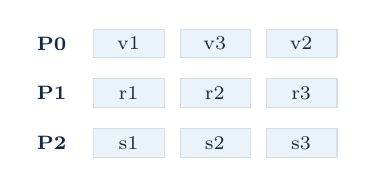
\begin{tikzpicture}[x=.80cm,y=.63cm]
\node[anchor=east,font=\scriptsize\bfseries,text=Navy] at (0,2.55) {P0};
\node[anchor=east,font=\scriptsize\bfseries,text=Navy] at (0,1.55) {P1};
\node[anchor=east,font=\scriptsize\bfseries,text=Navy] at (0,.55) {P2};
\foreach \y/\nums in {2.55/2,1.55/3,.55/2}{
  \foreach \x in {1,2,3}{\draw[Line,fill=Sky] ({(\x-1)*1.37+.28},\y-.29) rectangle ({(\x-1)*1.37+1.40},\y+.29);}
}
\node[font=\scriptsize,text=Dark] at (.83,2.55){v1};\node[font=\scriptsize,text=Dark] at (2.2,2.55){v3};\node[font=\scriptsize,text=Dark] at (3.57,2.55){v2};
\node[font=\scriptsize,text=Dark] at (.83,1.55){r1};\node[font=\scriptsize,text=Dark] at (2.2,1.55){r2};\node[font=\scriptsize,text=Dark] at (3.57,1.55){r3};
\node[font=\scriptsize,text=Dark] at (.83,.55){s1};\node[font=\scriptsize,text=Dark] at (2.2,.55){s2};\node[font=\scriptsize,text=Dark] at (3.57,.55){s3};
\end{tikzpicture}\par\smallskip
{\fontsize{9}{12}\selectfont\strong{Offset:} position within a partition.\par
Spark reads \texttt{config.snapshots} and checkpoints its progress.}
\end{tcolorbox}
\end{column}
\end{columns}
\vspace{.13cm}
\begin{tcolorbox}[colback=PaleGold,colframe=PaleGold]
\fontsize{9}{11}\selectfont\strong{Important:} Kafka partition order does not imply source-version order; keying by asset does not solve delayed/replayed source versions.
\end{tcolorbox}
\sourceline{messaging/kafka\_producer.py; docs/kafka-topics.md; spark/streaming/kafka\_source.py.}
\end{frame}

\begin{frame}{Boundary 2 / Spark: from bytes to meaningful changes}
\vspace{.07cm}
\centering
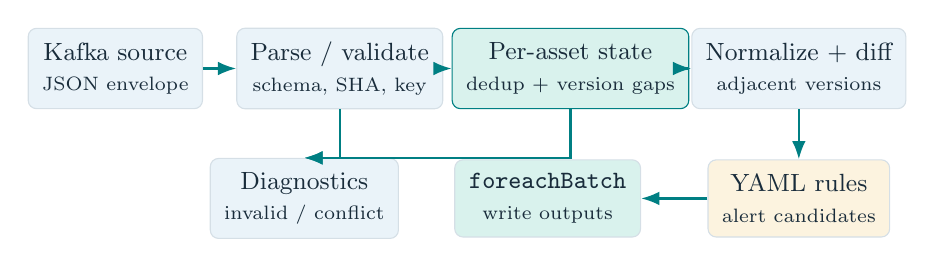
\begin{tikzpicture}[x=1cm,y=1cm,>=Latex]
\node[flow,fill=Sky,minimum width=2.04cm,minimum height=1.02cm] (a) at (1.18,3.08) {Kafka source\\\scriptsize JSON envelope};
\node[flow,fill=Sky,minimum width=2.16cm,minimum height=1.02cm] (b) at (4.03,3.08) {Parse / validate\\\scriptsize schema, SHA, key};
\node[tealflow,minimum width=2.24cm,minimum height=1.02cm] (c) at (6.96,3.08) {Per-asset state\\\scriptsize dedup + version gaps};
\node[flow,fill=Sky,minimum width=2.16cm,minimum height=1.02cm] (d) at (9.86,3.08) {Normalize + diff\\\scriptsize adjacent versions};
\draw[flowarrow] (a)--(b);\draw[flowarrow] (b)--(c);\draw[flowarrow] (c)--(d);
\node[flow,fill=PaleGold,minimum width=2.18cm,minimum height=.98cm] (e) at (9.86,1.43) {YAML rules\\\scriptsize alert candidates};
\node[flow,fill=Mint,minimum width=2.36cm,minimum height=.98cm] (f) at (6.67,1.43) {\texttt{foreachBatch}\\\scriptsize write outputs};
\node[flow,fill=Sky,minimum width=2.35cm,minimum height=.98cm] (g) at (3.58,1.43) {Diagnostics\\\scriptsize invalid / conflict};
\draw[flowarrow] (d.south)--(e.north);\draw[flowarrow] (e.west)--(f.east);
\draw[flowarrow] (b.south) |- (g.north);
\draw[flowarrow] (c.south) |- (g.north);
\end{tikzpicture}
\vspace{.12cm}
\begin{tcolorbox}[colback=White]
\fontsize{10}{12}\selectfont \strong{Why stateful?} Compare only $v_i \rightarrow v_{i+1}$ for the same asset, despite retries, duplicate IDs and late arrival order. Event-time watermark + eviction bound memory use.
\end{tcolorbox}
\sourceline{spark/streaming/main.py; validation.py; stateful.py; processing/{state,normalization,diff,rules}.py.}
\end{frame}

\begin{frame}[shrink=12]{Late arrivals: restore version order}
\vspace{.08cm}
\begin{tcolorbox}[colback=White]
\strong{Observed arrival order}\hfill\muted{Kafka messages may carry out-of-order source versions}
\vspace{.07cm}
\begin{center}
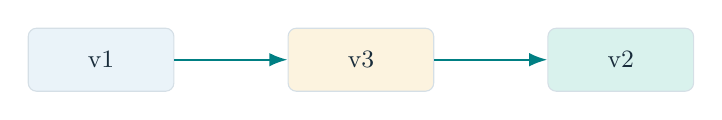
\begin{tikzpicture}[>=Latex]
 \node[flow,fill=Sky,minimum width=1.85cm] (x1) at (0,0) {v1};
 \node[flow,fill=PaleGold,minimum width=1.85cm] (x3) at (3.3,0) {v3};
 \node[flow,fill=Mint,minimum width=1.85cm] (x2) at (6.6,0) {v2};
 \draw[flowarrow] (x1)--(x3);
 \draw[flowarrow] (x3)--(x2);
\end{tikzpicture}
\end{center}
\end{tcolorbox}
\vspace{.10cm}
\begin{tcolorbox}[colback=Mint,colframe=Mint]
\strong{Stateful version matching}\hfill\muted{Per-asset bounded buffer}
\vspace{.09cm}
\begin{center}
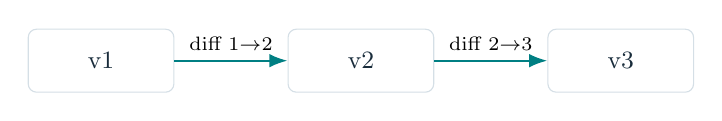
\begin{tikzpicture}[>=Latex]
 \node[flow,fill=White,minimum width=1.85cm] (x1) at (0,0) {v1};
 \node[flow,fill=White,minimum width=1.85cm] (x2) at (3.3,0) {v2};
 \node[flow,fill=White,minimum width=1.85cm] (x3) at (6.6,0) {v3};
 \draw[flowarrow] (x1)--node[above,font=\scriptsize]{diff 1$\to$2}(x2);
 \draw[flowarrow] (x2)--node[above,font=\scriptsize]{diff 2$\to$3}(x3);
\end{tikzpicture}
\end{center}
\end{tcolorbox}
\vspace{.12cm}
\begin{tcolorbox}[colback=White]
{\fontsize{10}{12}\selectfont\strong{Rule:} emit $(v_i,v_{i+1})$ only if both endpoints exist and that logical edge has not already been emitted.}\par
{\fontsize{8}{10}\selectfont\muted{Retention and watermark policies bound late repair; they do not make late-data recovery unlimited.}}
\end{tcolorbox}
\sourceline{processing/state.py; spark/streaming/stateful.py; scripts/kafka\_stateful\_demo.py.}
\end{frame}

\begin{frame}{Diffs become explainable alerts}
\vspace{.05cm}
\begin{columns}[T,onlytextwidth]
\begin{column}{.51\textwidth}
\begin{tcolorbox}[height=3.95cm,title=\strong{Version 10 $\rightarrow$ 11},colbacktitle=Sky]
{\ttfamily\fontsize{12}{17}\selectfont
\textcolor{Red}{- logging enabled}\\
\textcolor{Teal}{+ logging disabled}\\[3mm]
\textcolor{Red}{- telnet disabled}\\
\textcolor{Teal}{+ telnet enabled}}
\par\vspace{.35cm}
{\fontsize{9}{12}\selectfont Normalization removes selected textual noise and masks supported secret patterns before diffing.}
\end{tcolorbox}
\end{column}
\begin{column}{.47\textwidth}
\begin{tcolorbox}[height=1.87cm,colback=PaleGold,colframe=PaleGold]
\kicker{Rule match / high}\par\medskip\strong{Logging disabled}\par
{\fontsize{9}{11}\selectfont Regex on \texttt{added} diff lines}
\end{tcolorbox}
\vspace{.18cm}
\begin{tcolorbox}[height=1.87cm,colback=PaleRed,colframe=PaleRed]
\kicker{Rule match / critical}\par\medskip\strong{Telnet enabled}\par
{\fontsize{9}{11}\selectfont Regex on \texttt{added} diff lines}
\end{tcolorbox}
\end{column}
\end{columns}
\vspace{.15cm}
{\fontsize{10}{12}\selectfont\strong{Interpretation boundary:} a rule alert is not proof of an incident; line diff is not a vendor-semantic configuration parser.}
\sourceline{processing/demo.py; processing/diff.py; rules/default.yaml; processing/normalization.py.}
\end{frame}

\begin{frame}[shrink=12]{Boundary 3 / MinIO: how the Parquet history is laid out}
\vspace{.02cm}
\begin{columns}[T,onlytextwidth]
\begin{column}{.52\textwidth}
\begin{tcolorbox}[colback=White,height=3.96cm]
\kicker{One S3-compatible bucket}\par\medskip
{\ttfamily\fontsize{10}{14}\selectfont
config-lake/\\
\quad raw/snapshots/\\
\quad processed/snapshots/\\
\quad processed/diffs/\\
\quad processed/alerts/\\
\quad processed/diagnostics/\\
\quad analytics/\ldots}
\par\medskip
{\fontsize{9}{12}\selectfont\muted{Each micro-batch is scoped by query\_id/batch\_id; data files are partitioned by year/month/day.}}
\end{tcolorbox}
\end{column}
\begin{column}{.46\textwidth}
\begin{tcolorbox}[colback=Sky,colframe=Sky,height=1.85cm]
\kicker{Raw}\par\medskip
{\fontsize{10}{13}\selectfont Keep Kafka payload bytes with topic, partition and offset provenance.}
\end{tcolorbox}
\vspace{.17cm}
\begin{tcolorbox}[colback=Mint,colframe=Mint,height=1.92cm]
\kicker{Processed}\par\medskip
{\fontsize{10}{13}\selectfont Typed normalized snapshots, diffs, alerts and diagnostics stored as Snappy Parquet.}
\end{tcolorbox}
\end{column}
\end{columns}
\vspace{.13cm}
\begin{tcolorbox}[colback=PaleGold,colframe=PaleGold]
\fontsize{9}{11}\selectfont\strong{Three different partitions:} Kafka partition (event log), Spark execution partition (parallel tasks), and date partition (object paths).
\end{tcolorbox}
\sourceline{spark/streaming/sinks/lake.py; docs/data-lake.md; docs/pipeline-integrity-amendment.md.}
\end{frame}

\begin{frame}{Boundary 3 / Commit: make complete batches visible}
\vspace{.02cm}
\centering
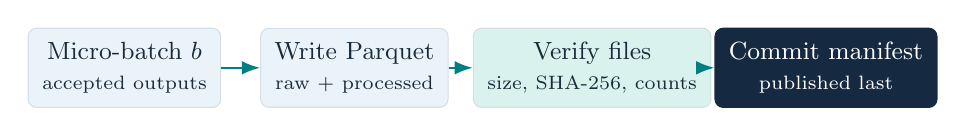
\begin{tikzpicture}[x=1cm,y=1cm,>=Latex]
\node[flow,fill=Sky,minimum width=2.10cm,minimum height=.9cm] (b) at (1.19,3.34) {Micro-batch $b$\\\scriptsize accepted outputs};
\node[flow,fill=Sky,minimum width=2.30cm,minimum height=.9cm] (w) at (4.11,3.34) {Write Parquet\\\scriptsize raw + processed};
\node[flow,fill=Mint,minimum width=2.30cm,minimum height=.9cm] (v) at (7.13,3.34) {Verify files\\\scriptsize size, SHA-256, counts};
\node[darkflow,minimum width=2.27cm,minimum height=.9cm] (m) at (10.10,3.34) {Commit manifest\\\scriptsize published last};
\draw[flowarrow] (b)--(w);\draw[flowarrow] (w)--(v);\draw[flowarrow] (v)--(m);
\end{tikzpicture}
\vspace{.20cm}
\begin{columns}[T,onlytextwidth]
\begin{column}{.49\textwidth}
\begin{tcolorbox}[height=2.28cm,colback=Mint,colframe=Mint]
\strong{What readers can trust}\par\medskip
{\fontsize{10}{13}\selectfont Manifest-declared, verified files form the accepted batch. Matching retry can be recognized; a partial write is not published as committed.}
\end{tcolorbox}
\end{column}
\begin{column}{.49\textwidth}
\begin{tcolorbox}[height=2.28cm,colback=PaleGold,colframe=PaleGold]
\strong{What still remains open}\par\medskip
{\fontsize{10}{13}\selectfont No atomic transaction across MinIO, Elasticsearch and Kafka. Kafka alerts can be physically duplicated on some retries.}
\end{tcolorbox}
\end{column}
\end{columns}
\sourceline{spark/streaming/sinks/lake.py; spark/streaming/outputs.py; docs/pipeline-integrity-amendment.md.}
\end{frame}

\begin{frame}[shrink=12]{Boundary 4 / Serving: one source of truth, two readers}
\vspace{.07cm}
\centering
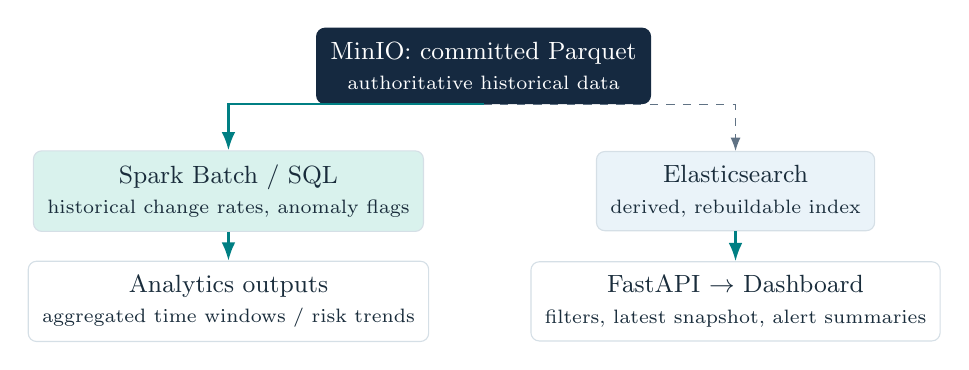
\begin{tikzpicture}[x=1cm,y=1cm,>=Latex]
\node[darkflow,minimum width=3.18cm,minimum height=.88cm] (lake) at (5.94,3.72) {MinIO: committed Parquet\\\scriptsize authoritative historical data};
\node[flow,fill=Mint,minimum width=3.37cm,minimum height=.85cm] (batch) at (2.7,2.13) {Spark Batch / SQL\\\scriptsize historical change rates, anomaly flags};
\node[flow,fill=Sky,minimum width=3.37cm,minimum height=.85cm] (elastic) at (9.14,2.13) {Elasticsearch\\\scriptsize derived, rebuildable index};
\draw[flowarrow] (lake.south) -| (batch.north);
\draw[-Latex,draw=Muted,dashed] (lake.south) -| (elastic.north);
\node[flow,fill=White,minimum width=3.37cm,minimum height=.85cm] (analytics) at (2.7,.73) {Analytics outputs\\\scriptsize aggregated time windows / risk trends};
\node[flow,fill=White,minimum width=3.37cm,minimum height=.85cm] (api) at (9.14,.73) {FastAPI $\rightarrow$ Dashboard\\\scriptsize filters, latest snapshot, alert summaries};
\draw[flowarrow] (batch.south)--(analytics.north);
\draw[flowarrow] (elastic.south)--(api.north);
\end{tikzpicture}
\vspace{.13cm}
\begin{tcolorbox}[colback=PaleGold,colframe=PaleGold]
\fontsize{9.5}{11.5}\selectfont\strong{Data boundary:} API is read-only and does not return raw configuration bodies. Dashboard cross-domain research cards come from accepted evidence bundles, not a unified live stream for all domains.
\end{tcolorbox}
\sourceline{docs/api.md; docs/historical-analytics.md; docs/elasticsearch.md; frontend/public/research/v1/catalog.json.}
\end{frame}

\begin{frame}[shrink=12]{From configuration history to four temporal contracts}
\vspace{.03cm}
\begin{columns}[T,onlytextwidth]
\begin{column}{.49\textwidth}
\begin{tcolorbox}[colback=White,height=1.72cm]
\kicker{Terraform / file versions}\par\smallskip
\strong{Adjacent version diff}\par
{\fontsize{9}{11}\selectfont Compare $v_i$ with $v_{i+1}$, not Git commits with deployments.}
\end{tcolorbox}
\vspace{.10cm}
\begin{tcolorbox}[colback=White,height=1.72cm]
\kicker{RIS / BGP occurrences}\par\smallskip
\strong{Preserve event multiplicity}\par
{\fontsize{9}{11}\selectfont A repeated announcement may be a separate real occurrence.}
\end{tcolorbox}
\end{column}
\begin{column}{.49\textwidth}
\begin{tcolorbox}[colback=White,height=1.72cm]
\kicker{RPKI / daily state}\par\smallskip
\strong{Set membership transitions}\par
{\fontsize{9}{11}\selectfont Differences between complete observed days, not operator actions.}
\end{tcolorbox}
\vspace{.10cm}
\begin{tcolorbox}[colback=White,height=1.72cm]
\kicker{DNS / measurement}\par\smallskip
\strong{Observed query responses}\par
{\fontsize{9}{11}\selectfont Vantage/coverage limits prohibit global-state claims.}
\end{tcolorbox}
\end{column}
\end{columns}
\vspace{.17cm}
\begin{tcolorbox}[colback=Mint,colframe=Mint]
\fontsize{10}{12}\selectfont\strong{What is shared:} Kafka/Spark execution, typed records, provenance, committed Parquet. \quad\strong{What differs:} identity, timing, dedup, and what a ``change'' means.
\end{tcolorbox}
\sourceline{frontend/public/research/v1/catalog.json; docs/phase20-cross-domain-analysis.md.}
\end{frame}

\begin{frame}[shrink=12]{Four processing lanes: shared platform, separate logic}
\vspace{.08cm}
\centering
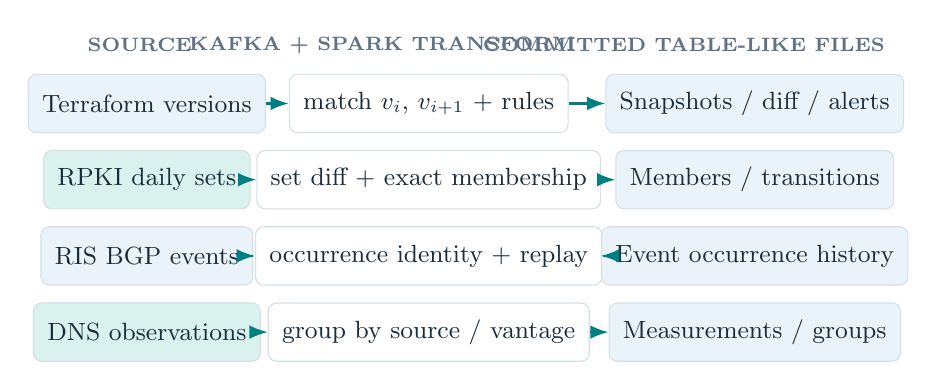
\begin{tikzpicture}[x=1cm,y=.88cm,>=Latex]
\node[font=\scriptsize\bfseries,text=Muted] at (1.13,4.72) {SOURCE};
\node[font=\scriptsize\bfseries,text=Muted] at (4.21,4.72) {KAFKA + SPARK TRANSFORM};
\node[font=\scriptsize\bfseries,text=Muted] at (8.04,4.72) {COMMITTED TABLE-LIKE FILES};
\foreach \id/\y/\src/\work/\out/\shade in {
  a/3.88/{Terraform versions}/{match $v_i$, $v_{i+1}$ + rules}/{Snapshots / diff / alerts}/Sky,
  b/2.78/{RPKI daily sets}/{set diff + exact membership}/{Members / transitions}/Mint,
  c/1.68/{RIS BGP events}/{occurrence identity + replay}/{Event occurrence history}/Sky,
  d/.58/{DNS observations}/{group by source / vantage}/{Measurements / groups}/Mint}{
 \node[flow,fill=\shade,minimum width=2.13cm,minimum height=.74cm] (s\id) at (1.22,\y) {\src};
 \node[flow,fill=White,minimum width=3.38cm,minimum height=.74cm] (w\id) at (4.80,\y) {\work};
 \node[flow,fill=Sky,minimum width=2.69cm,minimum height=.74cm] (o\id) at (8.94,\y) {\out};
 \draw[flowarrow] (s\id.east)--(w\id.west);
 \draw[flowarrow] (w\id.east)--(o\id.west);
}
\end{tikzpicture}
\vspace{.16cm}
\begin{tcolorbox}[colback=PaleGold,colframe=PaleGold]
\fontsize{9}{11}\selectfont\strong{Not one universal diff algorithm:} configuration rules apply to the versioned file lane. RIS, RPKI and DNS use separate domain definitions and proof obligations.
\end{tcolorbox}
\sourceline{spark/streaming/; spark/rpki\_stream.py; spark/ris.py; spark/dns.py; docs/architecture.md.}
\end{frame}

\begin{frame}[shrink=12]{Prepared data: accepted measurements, not mixed units}
\vspace{.04cm}
\begin{columns}[T,onlytextwidth]
\begin{column}{.49\textwidth}
\bigstat{10,188}{Terraform accepted Git versions / 375 repos}{Sky}
\vspace{.16cm}
\bigstat{4,725,156}{RIS event occurrences / 1 hour / rrc00}{Mint}
\end{column}
\begin{column}{.49\textwidth}
\bigstat{14}{Complete RPKI daily observations / 1--14 Sep}{Sky}
\vspace{.16cm}
\bigstat{2,234,863}{Raw DNS measurements / two source objects}{Mint}
\end{column}
\end{columns}
\vspace{.18cm}
\begin{tcolorbox}[colback=PaleGold,colframe=PaleGold]
\fontsize{9.8}{12}\selectfont\strong{Never sum these rows:} file revisions, full daily state sets, event occurrences and measurements are different units. Controlled synthetic histories test retries and late delivery.
\end{tcolorbox}
\sourceline{frontend/public/research/v1/catalog.json; accepted scope fixed per source and time window.}
\end{frame}

\begin{frame}[shrink=12]{What is implemented: executable and integrated evidence}
\vspace{.07cm}
\begin{columns}[T,onlytextwidth]
\begin{column}{.49\textwidth}
\begin{tcolorbox}[colback=Sky,colframe=Sky,height=3.67cm]
\kicker{Runnable processing demonstration}\par\medskip
{\ttfamily\fontsize{11}{16}\selectfont
make setup\\
make processing-demo}
\par\vspace{.35cm}
{\fontsize{25}{27}\selectfont\color{Navy}\bfseries 178}\par
{\fontsize{9}{12}\selectfont state, diff and rule unit tests passed, as recorded for 25 Oct 2026.}
\end{tcolorbox}
\end{column}
\begin{column}{.49\textwidth}
\begin{tcolorbox}[colback=Mint,colframe=Mint,height=3.67cm]
\kicker{Previously recorded local replay}\par\medskip
{\fontsize{19}{22}\selectfont\bfseries 10,188} \quad {\fontsize{9}{11}\selectfont snapshots}\par\vspace{.20cm}
{\fontsize{19}{22}\selectfont\bfseries 3,683} \quad {\fontsize{9}{11}\selectfont adjacent diffs}\par\vspace{.20cm}
{\fontsize{19}{22}\selectfont\bfseries 29.4 MB} \quad {\fontsize{9}{11}\selectfont Parquet committed}\par\smallskip
{\fontsize{9}{12}\selectfont Kafka $\rightarrow$ Spark $\rightarrow$ MinIO; 375 scoped Terraform repositories.}
\end{tcolorbox}
\end{column}
\end{columns}
\vspace{.15cm}
\begin{tcolorbox}[colback=PaleGold,colframe=PaleGold]
\fontsize{9.5}{11}\selectfont\strong{Do not conflate:} the small Python demo needs no services; the integrated replay is a prior accepted local run, not a fresh live checkpoint test.
\end{tcolorbox}
\sourceline{presentation README; docs/phase12-acceptance.md. 29,402,997 committed Parquet bytes.}
\end{frame}

\begin{frame}[shrink=12]{One focused result: RPKI representation trade-off}
\vspace{.03cm}
\begin{columns}[T,onlytextwidth]
\begin{column}{.55\textwidth}
\kicker{Same 14 complete daily observations}\par\medskip
{\fontsize{9.8}{12}\selectfont
\strong{R1} Full daily states\par
\strong{R2} Initial state + daily additions/removals\par
\strong{R3} R2 + extra full state on day 8}
\par\vspace{.21cm}
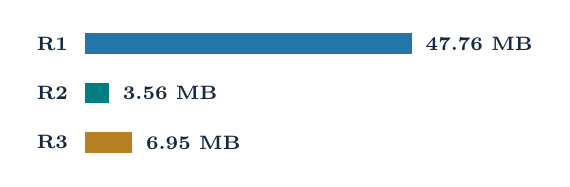
\begin{tikzpicture}[x=.087cm,y=.71cm]
\foreach \i/\name/\val/\barcol in {0/R1/47.76/Blue,1/R2/3.56/Teal,2/R3/6.95/Gold}{
\pgfmathsetmacro{\yy}{2.35-\i*.88}
\node[anchor=east,font=\scriptsize\bfseries,text=Navy] at (-1,\yy+.19) {\name};
\fill[\barcol] (0,\yy) rectangle (\val,\yy+.37);
\node[anchor=west,font=\scriptsize\bfseries,text=Navy] at (\val+.6,\yy+.18) {\val\ MB};
}
\end{tikzpicture}
\par\vspace{.10cm}{\fontsize{8.5}{10}\selectfont\color{Muted}Warm reconstruction (R1/R2/R3): 6.73 / 6.88 / 6.76 s.}
\end{column}
\begin{column}{.43\textwidth}
\begin{tcolorbox}[colback=Mint,colframe=Mint,height=2.05cm]
\kicker{Analytical files only}\par\medskip
{\fontsize{23}{26}\selectfont\color{Navy}\bfseries --92.6\%}\par
{\fontsize{9}{11}\selectfont R2 vs R1 (47.76 $\rightarrow$ 3.56 MB)}
\end{tcolorbox}
\vspace{.15cm}
\begin{tcolorbox}[colback=PaleGold,colframe=PaleGold,height=2.03cm]
\kicker{All measured local files}\par\medskip
{\fontsize{23}{26}\selectfont\color{Navy}\bfseries --17.5\%}\par
{\fontsize{9}{11}\selectfont R2 vs R1 (251.98 $\rightarrow$ 207.90 MB)}
\end{tcolorbox}
\end{column}
\end{columns}
\sourceline{workloads/results/phase20/rpki-representations.json and rpki-all-in-storage.json; excludes deployed broker/checkpoint bytes.}
\end{frame}

\begin{frame}[shrink=12]{Architecture guarantees versus unproven claims}
\vspace{.04cm}
\begin{columns}[T,onlytextwidth]
\begin{column}{.49\textwidth}
\begin{tcolorbox}[colback=Mint,colframe=Mint,height=3.65cm]
\kicker{Validated within accepted scope}\par\medskip
{\fontsize{10.3}{15}\selectfont
\textbullet\ Deterministic version adjacency / rules\\[4pt]
\textbullet\ Committed Parquet and integrity checks\\[4pt]
\textbullet\ Scoped historical replay and exact reads\\[4pt]
\textbullet\ Separate temporal contracts for four sources}
\end{tcolorbox}
\end{column}
\begin{column}{.49\textwidth}
\begin{tcolorbox}[colback=PaleGold,colframe=PaleGold,height=3.65cm]
\kicker{Not yet established}\par\medskip
{\fontsize{10.3}{15}\selectfont
\textbullet\ Multi-node horizontal scaling or HA\\[4pt]
\textbullet\ Cross-sink end-to-end exactly-once\\[4pt]
\textbullet\ Production traffic realism or device impact\\[4pt]
\textbullet\ Storage savings across every domain}
\end{tcolorbox}
\end{column}
\end{columns}
\vspace{.19cm}
\begin{tcolorbox}[colback=White]
\fontsize{9.5}{12}\selectfont\strong{Checkpoint conclusion:} executable architecture with bounded correctness evidence; not a demonstrated production-scale configuration management service.
\end{tcolorbox}
\sourceline{docs/phase12-acceptance.md; docs/phase20-acceptance.md; docs/phase20-k8s-acceptance.md.}
\end{frame}

\begin{frame}[shrink=12]{Checkpoint readiness and next milestone}
\vspace{.05cm}
\begin{columns}[T,onlytextwidth]
\begin{column}{.49\textwidth}
\kicker{Required at this checkpoint}\par\medskip
\begin{tcolorbox}[colback=White]\strong{Source code}\par{\fontsize{9}{11}\selectfont Runnable generator / processing demo, automated tests}\end{tcolorbox}
\vspace{.12cm}
\begin{tcolorbox}[colback=White]\strong{Data readiness}\par{\fontsize{9}{11}\selectfont Four scoped real-source corpora and manifests}\end{tcolorbox}
\vspace{.12cm}
\begin{tcolorbox}[colback=White]\strong{System architecture}\par{\fontsize{9}{11}\selectfont Kafka, four Spark paths, MinIO and serving boundary}\end{tcolorbox}
\end{column}
\begin{column}{.49\textwidth}
\kicker{Next milestone: evaluation}\par\medskip
\begin{tcolorbox}[colback=Sky,colframe=Sky]\strong{01. Integrated reproducible demo}\par{\fontsize{9}{11}\selectfont Source $\rightarrow$ Kafka $\rightarrow$ committed Parquet $\rightarrow$ API}\end{tcolorbox}
\vspace{.12cm}
\begin{tcolorbox}[colback=Sky,colframe=Sky]\strong{02. Sustained workload tests}\par{\fontsize{9}{11}\selectfont Logical throughput, latency, backlog, memory, storage}\end{tcolorbox}
\vspace{.12cm}
\begin{tcolorbox}[colback=Sky,colframe=Sky]\strong{03. Failure / restart evidence}\par{\fontsize{9}{11}\selectfont Replay and checkpoint behavior on latest revision}\end{tcolorbox}
\end{column}
\end{columns}
\vspace{.13cm}
\begin{center}{\fontsize{13}{16}\selectfont\color{Teal}\bfseries Questions and feedback welcome}\end{center}
\sourceline{https://github.com/kongwoang/ConfigStream; checkpoint scope: local / one-node accepted demonstrations.}
\end{frame}

\end{document}
